\begin{figure}[H]
\begin{minipage}[ct]{0.47\textwidth}

\begin{center}
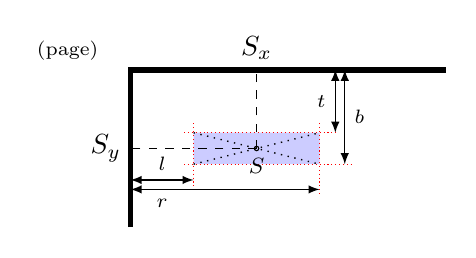
\begin{tikzpicture}[fill=blue!20, scale=0.4]

% Koordinaten/Beschriftungen
\draw[line width=2pt] (0,-5) -- (0,0) -- (10,0);
\draw (-2,0) node[anchor=south]{\scriptsize (\code{page})};
%\draw (0,-0.6) node[anchor=east]{\scriptsize \code{page} (links)};

% Element
\fill (2,-2) -- (6,-2) -- (6,-3) -- (2,-3) -- (2,-2);

% Pfeile horizontal
\draw[>=latex,<->] (0,-3.5) -- (2, -3.5);
\draw[>=latex,<->] (0,-3.8) -- (6, -3.8);
\draw (1, -3.5) node[anchor=south]{{\scriptsize $l$}};
\draw (1, -3.8) node[anchor=north]{{\scriptsize $r$}};

% Pfeile vertikal
\draw[>=latex,<->] (6.5,0) -- (6.5, -2);
\draw[>=latex,<->] (6.8,0) -- (6.8, -3);
\draw (6.5, -1) node[anchor=east]{{\scriptsize $t$}};
\draw (6.8, -1.5) node[anchor=west]{{\scriptsize $b$}};

% Hilfslinien
\draw[red, densely dotted] (1.7,-2) -- (6.6,-2);
\draw[red, densely dotted] (1.7,-3) -- (7.1,-3);
\draw[red, densely dotted] (2,-1.7) -- (2,-3.7);
\draw[red, densely dotted] (6,-1.7) -- (6,-4);

% Diag
\draw (4,-2.5) circle (2pt);
\draw[dotted, line width=0.5pt] (2,-2) -- (6,-3);
\draw[dotted, line width=0.5pt] (2,-3) -- (6,-2);
\draw (4,-2.5) node[anchor=north]{{\footnotesize $S$}};

% Koordinaten
\draw[dashed] (4,-2.5) -- (4,0) node[anchor=south]{$S_x$};
\draw[dashed] (4,-2.5) -- (0,-2.5) node[anchor=east]{$S_y$};
\end{tikzpicture}

		
\begin{eqnarray*}
	S_{xy}	&=& \left(\frac{r+l}{2}, \frac{t+b}{2}\right)
\end{eqnarray*}		

\end{center}
\end{minipage}
\begin{minipage}[ct]{0.47\textwidth}

\begin{center}
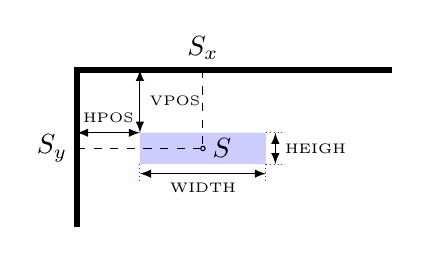
\begin{tikzpicture}[fill=blue!20, scale=0.4]
% Koordinaten/Beschriftungen
\draw[line width=2pt] (0,-5) -- (0,0) -- (10,0);
% \draw (-2,0) node[anchor=south]{\scriptsize \code{page}};

% Element
\fill (2,-2) -- (6,-2) -- (6,-3) -- (2,-3) -- (2,-2);

\draw[>=latex,<->] (2,0) -- (2,-2);
\draw (2,-1) node[anchor=west]{{\tiny VPOS}};
\draw[>=latex,<->] (0,-2) -- (2,-2);
\draw (1,-2) node[anchor=south]{{\tiny HPOS}};
\draw[>=latex,<->] (2,-3.3) -- (6,-3.3);
\draw (4,-3.3) node[anchor=north]{{\tiny WIDTH}};
\draw[>=latex,<->] (6.3,-2) -- (6.3,-3);
\draw (6.3,-2.5) node[anchor=west]{{\tiny HEIGH}};

\draw[red, densely dotted] (2,-3)--(2,-3.5);
\draw[red, densely dotted] (6,-3)--(6,-3.5);
\draw[red, densely dotted] (6,-3)--(6.5,-3);
\draw[red, densely dotted] (6,-2)--(6.5,-2);

\draw[dashed] (4,0)--(4,-2.5);
\draw[dashed] (0,-2.5)--(4,-2.5);

\draw (4,0) circle (2pt);
\draw (4,-2.5) circle (2pt);
\draw (0,-2.5) circle (2pt);

\draw (4,0) node[anchor=south]{$S_x$};
\draw (4,-2.5) node[anchor=west]{$S$};
\draw (0,-2.5) node[anchor=east]{$S_y$};

\end{tikzpicture}

\begin{eqnarray*}
S_{xy} = \left(\text{HPOS}+\frac{\text{WIDTH}}{2}, \text{VPOS}+\frac{\text{HEIGHT}}{2}\right)
\end{eqnarray*}	
\end{center}

\end{minipage}
\caption{Schwerpunktskoordinaten $S_{xy}$ von Elementen in Version 1 (links) und 2.}
\label{fig:Schwerpunkte}
\end{figure}